\section{Introduction}
\paragraph{Primary Text Reading.} \citeA[chap. 1]{tsay2005aft}\index{Tsay, Ruey}
\subsection{What is \fts{} analysis?}\index{Time Series!definition}
In general, a time series is a sequence of data points, usually measured at successive times, spaced at specific intervals. Time series analysis comprises methods that seek to understand the context of the data points to answer questions such as, ``What is this series telling me about whatever is generating this series?'', or to make \emph{forecasts} to predict future data points.
\marginpar{\begin{small}\begin{flushleft}\textcolor{blue}{Much of time series analysis is predicting future outcomes.}\end{flushleft}\end{small}}
Time series forecasting is the use of a model to forecast future events based on known past events: to forecast future data points before they occur. A good example might be forecasting a price of a share of stock based on its past performance.

Financial time series analysis is concerned with asset valuation and volatility over time. The state of the world today (\textit{e.g.} a stock price or interest rate) is affected in some way by the previous state, perhaps yesterday or two seconds ago. Similarly, the state of the world in the future is likely to be affected by the current state. This assumption allows some level of \emph{financial forecasting} using various methods of time series analysis.

There are three major outcomes of time series analysis, graphical analysis, autocorrelation, and trend behavior. We will briefly discuss how each is explored.

\paragraph{Graphical analysis.} When we view a time series in the form of time series plot, we may observe peaks and valleys. It may become apparent that a trend has developed by looking at the rising and falling of the line. Methods that analyze time series data graphically comprise \index{Technical Analysis}\emph{technical analysis} and a \index{Exploratory Data Analysis}\emph{Exploratory Data Analysis}.

\paragraph{Autocorrelation.}\index{Autocorrelation} We may want to measure the extend to which data points seem to rely upon previous points, or how random they seem to be. This type of analysis applies autocorrelation studies.

\paragraph{Trend behavior.} Some \fts{} exhibit trends which can be examined numerically. They may have some seasonal pattern, such that, for instance, their level will rise in summer and decline in winter.

\subsection{Review of matrices, statistics and probability }
\subsubsection{Descriptive Statistics}
This section is a brief review of inferential statistics and probability.  There will also be some review of linear algebra, the mathematics of matrices.

\marginpar{\begin{small}\begin{flushleft}\textcolor{red}{A working knowledge of statistics and matrix math is assumed.}\end{flushleft}\end{small}}
Descriptive statistics are used to describe the basic features of the data in a study. They provide simple summaries about the sample and the measures. Together with simple graphics analysis, they form the basis of virtually every quantitative analysis of data. Statistics such as mean, median, and standard deviation are descriptive.

Descriptive statistics are typically distinguished from \emph{inferential statistics}. With descriptive statistics we are simply describing what is or what the data shows. With inferential statistics, we are trying to reach conclusions that extend beyond the immediate data alone. For instance, we use inferential statistics to try to infer from the sample data what the population might think. Or, we use inferential statistics to make judgments of the probability that an observed difference between groups is a dependable one or one that might have happened by chance in this study. Thus, we use inferential statistics to make inferences from our data to more general conditions; we use descriptive statistics simply to describe what's going on in our data.

Every time we try to describe a large set of observations with a single indicator we run the risk of distorting the original data or losing important detail. For this reason, statistics such as kurtosis and skewness are helpful in describing a frequency distribution with respect to a normal distribution.

The normal distribution is a histogram depicting the probability of a number with respect to its distance from a mean of zero across a range $(- \infty , \infty)$.

\begin{equation}
\phi(z) = \frac{1}{\sqrt{2 \pi}} \exp(-z^2/2), \quad - \infty < z < \infty
\label{eq:pdf}
\end{equation}

For instance,  \eqref{eq:pdf} is the equation that produces Figure~\ref{figure:pdf}.
The cumulative distribution \eqref{eq:cdf} is depicted in Figure~\ref{figure:cdf}.

\begin{equation}
\phi(z) = \int^z_{-\infty} \frac{1}{\sqrt{2 \pi}} \exp(-z^2/2), \quad - \infty < z < \infty
\label{eq:cdf}
\end{equation}

\begin{figure}[t]
  \centering
  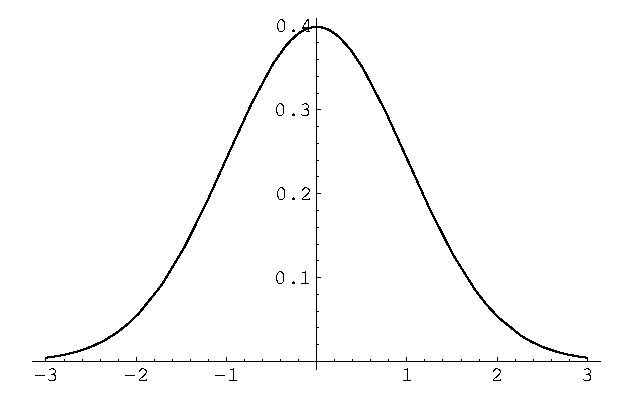
\includegraphics[scale=.75]{pdf}
  \caption{Normal Probability Density}
  \label{figure:pdf}
\end{figure}

\begin{figure}[t]
  \centering
  \includegraphics[scale=.75]{cdf}
  \caption{Normal Cumulative Distribution}
  \label{figure:cdf}
\end{figure}

A great deal of statistical analysis comes from the normal distribution. Being able to calculate the values of specific ranges in the distribution is essential to understanding descriptive statistics.

\subsubsection{Sampling and Validity}\index{Sampling}\index{Sampling!Validity}
Sampling is the process of selecting units (\textit{e.g.}, people, organizations) from a population of interest so that by studying the sample we may fairly generalize our results back to the population from which they were chosen. We begin by covering some of the key terms in sampling like ``population'' and ``sampling frame.'' Then, because some types of sampling rely upon quantitative models, we talk about some of the statistical terms used in sampling.

\paragraph{Random Sample.}\index{Sampling!Random}\index{Recursion|see{Recursion}}
Since it is not practical or even possible in many cases, to gather all data from a population, gathering a sample is preferred. However, the method by which a sample is chosen is very important and will affect the results of analysis. One of the easiest sampling methods is creating a \emph{random sample}.

How do we select a simple random sample? Assume that we are doing some research in equity analysis using a specific price forecasting method. First, we have to get the sampling frame organized. To accomplish this, we have to define the universe of stocks that are eligible for study. Next, we actually draw the sample using some random number assigned to each stock. If we are studying 100 stocks in our sample of perhaps 5,000 stocks. Then, the sampling fraction is $f = n/N = 100/5000 = .02$ or 2\%. To actually draw the sample, we have several options. We could print the list of 5,000 stocks, tear them into separate strips, put the strips in a box, and pull out the first 100. This mechanical procedure is tedious and the quality of the sample would depend on how thoroughly we mixed them up and how randomly we reached in.

A better procedure would be to use a random number generator that picks a number from 1 to 5,000, such as the following MATLAB code,\\

\ecaption{Generating 5,000 Random Integers}
\texttt{my\_sample=floor(5000*rand(1,100));} \\

However, this method does \emph{not} guarantee that the numbers generated will be unique, but it is a start.

Simple random sampling is simple to accomplish and is easy to explain to others. Because simple random sampling is a fair way to select a sample, it is reasonable to generalize the results from the sample back to the population. Simple random sampling is not the most statistically efficient method of sampling and we may, just because of the luck of the draw, not get good representation of subgroups in a population. To deal with these issues, we have to turn to other sampling methods.

\paragraph{Systematic Sample.} \index{Sampling!Systematic}
Another random selection method is to pick every $k$th item in a population.
Here are the steps to achieve a systematic random sample,
\begin{enumerate}
\item number the units in the population from 1 to $N$
\item decide on the $n$ (sample size) that we need
\item $k = N/n = $ the interval size
\item randomly select an integer between 1 to $k$
\item select every $k$th unit
\end{enumerate}

All of this will be much clearer with an example. Assume that we have a population that only has $N=100$ items in it and that we want to take a sample of $n=20$. To use systematic sampling, the population must be listed in a random order. The sampling fraction would be $f = 20/100 = 20\%$. In this case, the interval size, $k$, is equal to $N/n = 100/20 = 5$. Now, we select a random integer from 1 to 5. In our example, imagine that we chose 4. Now, to select the sample, we start with the 4th unit in the list and take every $k$th unit (every 5th, because $k$=5). We would be sampling units 4, 9, 14, 19, \ldots, 100 and we would have 20 units in our sample.

For this to work, it is essential that the units in the population are randomly ordered, at least with respect to the characteristics we are measuring. Systematic random sampling is fairly easy to do. We only have to select a single random number to start things off. It may also be more precise when selecting the sample size $n$ than a simple random sampling, which uses a random number generator that is not guaranteed to be unique.

\paragraph{Stratified Sample.} \index{Sampling!Stratified}
This is a sample within a sample because a sample is drawn, and then a sample from within that is drawn. Stratified random sampling, also sometimes called \emph{proportional} or \emph{quota random sampling}, involves dividing our population into homogeneous subgroups and then taking a simple random sample in each subgroup.

In more formal terms, we divide the population into non-overlapping groups (\textit{i.e.}, strata) $N_1, N_2, N_3, \ldots, N_i$, such that $N_1 + N_2 + N_3 + \cdots + N_i = N$. Then we select a simple random sample of $f = n/N$ in each strata.

There are several major reasons why we might prefer stratified sampling over simple random sampling. First, it assures that we will be able to represent not only the overall population, but also key subgroups of the population, especially small minority groups. If we want to be able to talk about subgroups, this may be the only way to effectively assure we will be able to.

If the subgroup is extremely small, we can use different sampling fractions, $f$ within the different strata to randomly over-sample the small group (although we will have to weight the within-group estimates using the sampling fraction whenever we want overall population estimates). When we use the same sampling fraction within strata we are conducting proportionate stratified random sampling. When we use different sampling fractions in the strata, we call this \emph{disproportionate stratified random sampling}.

Second, stratified random sampling will generally have more statistical precision than simple random sampling. This will only be true if the strata or groups are homogeneous. If they are, we expect that the variability within-groups is lower than the variability for the population as a whole. Stratified sampling capitalizes on that fact.

For example, we want to test a trading strategy that works well for stocks of consumer staples, automotive, and leisure industry. We have three populations. Let us say that the population of stocks for our study can be divided into three groups: consumer staples, automotive, and leisure. Furthermore, let us assume that both the automotive and the leisure stocks are relatively few within the population (10\% and 5\% respectively). If we just did a simple random sample of $n=100$ with a sampling fraction of 10\%, we would expect by chance alone that we would only get 10 and 5 persons from each of our two smaller groups. And, by chance, we might get fewer than that.

If we stratify, we can do better. First, let us determine how many stocks we want to have in each group. Let us say we still want to take a sample of 100 from the population of 1,000 stocks. But we think that in order to say anything about subgroups we will need at least 25 cases in each group. So, we will sample 50 consumer staples, 25 automotive, and 25 leisure stocks. We know that 10\% of the population, or 100 stocks, are automotive. If we randomly sample 25 of these, we have a within-stratum sampling fraction of $25/100 = 25\%$. Similarly, we know that 5\% or 50 stocks are leisure. So our within-stratum sampling fraction will be $25/50 = 50\%$. Finally, by subtraction we know that there are 850 consumer staples stocks. Our within-stratum sampling fraction for them is $50/850 =  5.88\%$. Because the groups are more homogeneous within-group than across the population as a whole, we can expect greater statistical precision (less variance). And, because we stratified, we know we will have enough cases from each group to make meaningful subgroup inferences.

\begin{table}[htbp]
   \centering
   \begin{tabular}{@{} lrcl @{}}
      \toprule
      \multicolumn{4}{c}{Stratified Sample} \\
      \hline
       Type    & within pop. & sample size & within-stratum sample \\
      \hline
      consumer staples  & 85\% & 50 & 50/850 = 5.88\% \\
      automotive   & 10\% & 25 & 25/100 = 25\% \\
      leisure industry & 5\%  & 25 & 25/50 = 50\% \\
      \bottomrule
   \end{tabular}
   \caption{Stratified Sample Selection}
   \label{tab:strat-sample}
\end{table}

\paragraph{Convenience Sample.}\index{Sampling!Convenience}
A convenience sample is one where the items sampled from the population are chosen for their easy access. For instance, a consumer survey conducted by asking the first 100 people who walk into a particular bank one morning is a convenience sample. Those not going to that bank on that morning are not part of the sample. This might be an important issue, or it might not be, depending upon the purpose of the survey. Choosing 100 stocks for analysis based upon the fact that the analyst has heard of them is also a convenience sample because it ignores the perhaps thousands of stocks unknown to the analyst.

\paragraph{Validity.}\index{Validity!External}
\emph{External validity} is related to generalizing.
\marginpar{\begin{small}\begin{flushleft}\textcolor{blue}{Validity refers to the approximate truth of propositions, inferences, or conclusions}\end{flushleft}\end{small}}
External validity refers to the approximate truth of conclusions that involve generalizations. In other words, external validity is the degree to which the conclusions in a study would hold for other persons in other places and at other times.

In science there are two major approaches to how we provide evidence for a generalization. The first approach is the \emph{Sampling Model}.\index{Validity!Sampling}
In the sampling model, we start by identifying the population to generalize to. Then, we draw a fair sample from that population and conduct research with the sample. Finally, because the sample is representative of the population, one can automatically generalize results back to the population. However, there are several problems with this approach.

First, perhaps we do not know at the time of the study who we might ultimately like to generalize to. Second, we may not be easily able to draw a fair or representative sample. Third, it is impossible to sample across all times that we might like to generalize to (like next year).

The second approach to generalizing is the \emph{Proximal Similarity Model}.\index{Validity!Proximal Similarity}
Under this model, we begin by thinking about different generalizability contexts and developing a theory about which contexts are more like our study and which are less so. For instance, we might imagine several settings that have people who are more similar to the people in our study or people who are less similar. This also holds for times and places.

When we place different contexts in terms of their relative similarities, we can call this implicit theoretical a gradient of similarity. Once we have developed this proximal similarity framework, we are able to generalize. How? We conclude that we can generalize the results of our study to other persons, places or times that are \emph{more like} (that is, more proximally similar) to our study. Notice that here, we can never generalize with certainty -- it is always a question of more or less similar.

\paragraph{Threats to External Validity.}
A threat to external validity is an explanation of how we might be wrong in making a generalization. For instance, we conclude that the results of our study (which was done in a specific place, with certain types of people, and at a specific time) can be generalized to another context (for instance, another place, with slightly different people, at a slightly later time). There are three major threats to external validity because there are three ways we could be wrong -- people, places or times.

Our critics could argue that the results of our study are due to the unusual type of people who were in the study. Or, they could argue that it might only work because of the unusual place we did the study in (perhaps we did our educational study in a college town with lots of high-achieving educationally-oriented students). Or, one might suggest that we did our study in a peculiar time. For instance, if we did an interest rate study the week after the Federal Reserve issues the well-publicized results of the latest rate change, we might get different results than if we had done it the week before.

\paragraph{Improving External Validity.}
How can we improve external validity? One way, based on the sampling model, suggests that we do a good job of drawing a sample from a population. For instance, we should use random selection, if possible, rather than a \emph{nonrandom} procedure.
\marginpar{\begin{small}\begin{flushleft}\textcolor{blue}{External validity (ability to generalize) will be stronger the more we replicate our study.}\end{flushleft}\end{small}}

A second approach would be to use the theory of proximal similarity more effectively. How? Perhaps we could do a better job of describing the ways our contexts and others differ, providing lots of data about the degree of similarity between various groups of people, places, and even times. We might even be able to map out the degree of proximal similarity among various contexts with a methodology like concept mapping. Perhaps the best approach to criticisms of generalizations is simply to show them that they are wrong -- do the study in a variety of places, with different people and at different times.

Once we identify the theoretical and accessible populations, we have to get a list of the members of the accessible population. The listing of the accessible population from which we draw our sample is called the \emph{sampling frame}. If we were doing a performance survey of S\&P 500 stocks, then the stocks within the index would be our sampling frame. Getting that listing is simply a matter of going to a Bloomberg terminal\index{Bloomberg}
and obtaining the list. Other studies may be as simple, such as studying the rate of inflation on the money supply, for instance. However, preparing sample data of credit default swaps, for which the data is very difficult to obtain, also is difficult to compare to other swaps. This is a generally inaccessible population.

People often confuse what is meant by \emph{random selection} with the idea of \emph{random assignment}. You should make sure that you understand the distinction between random selection and random assignment. Random selection is the method by which the sample is selected, and random assignment is the method by which those samples are assigned to a test group or to a control group.

\subsubsection{Inferential Statistics}
With inferential statistics, we are trying to reach conclusions that extend beyond the immediate data alone. For instance, we use inferential statistics to try to infer from the sample data what the population might signify. Or, we use inferential statistics to make judgments of the probability that an observed difference between groups is a dependable one or one that might have happened by chance in this study. Thus, we use inferential statistics to make inferences from our data to more general conditions; we use descriptive statistics simply to describe what is going on in our data.
\marginpar{\begin{small}\begin{flushleft}\textcolor{blue}{Inferential statistics help make predictions and judgements}\end{flushleft}\end{small}}

Most of the major inferential statistics come from a general family of statistical models known as the General Linear Model. This includes the $t$ test, Analysis of Variance (ANOVA), Analysis of Covariance (ANCOVA), regression analysis, and many of the multivariate methods like factor analysis, multidimensional scaling, cluster analysis, and discriminant function analysis.

The purpose of these statistical tests is to conduct an experiment. Is a certain procedure effective in forecasting rates? Is there a significant difference between two samples?

\subsection{Statistical Inference}\index{Statistical Inference}
When we make some conclusion from a data sample we obtained, we draw an inference about a population based on some statistical inference method. We may be attempting to predict one of the following,
\begin{itemize}
\item point estimate: \index{Point Estimation} we are trying to determine a specific number
\item interval estimate:\index{Interval Estimation} we are tying to obtain a \emph{confidence interval}
\item hypothesis test:\index{Hypothesis Test}  we run a statistical significance test to determine if a sample belongs in the population
\end{itemize}

\subsubsection{Point Estimation}\index{Point Estimation}
Point estimation involves the use of sample data to calculate a single value (known as a \emph{statistic}) which is to serve as a ``best guess'' for an unknown (fixed or random) population \emph{parameter}.
\marginpar{\begin{small}\begin{flushleft}\textcolor{red}{A statistic is drawn from a sample. \\ A parameter is contained in the population.}\end{flushleft}\end{small}}
One of the best known methods of point estimation is linear regression using the method of ordinary least squares. For example, Figure~\ref{figure:pt-est} is a linear regression through a scatterplot.

In most types of regression analysis, linear or otherwise, we are getting a point estimate through a plane, or more simply, a line that predicts points along the line.
\begin{figure}[t]
  \centering
  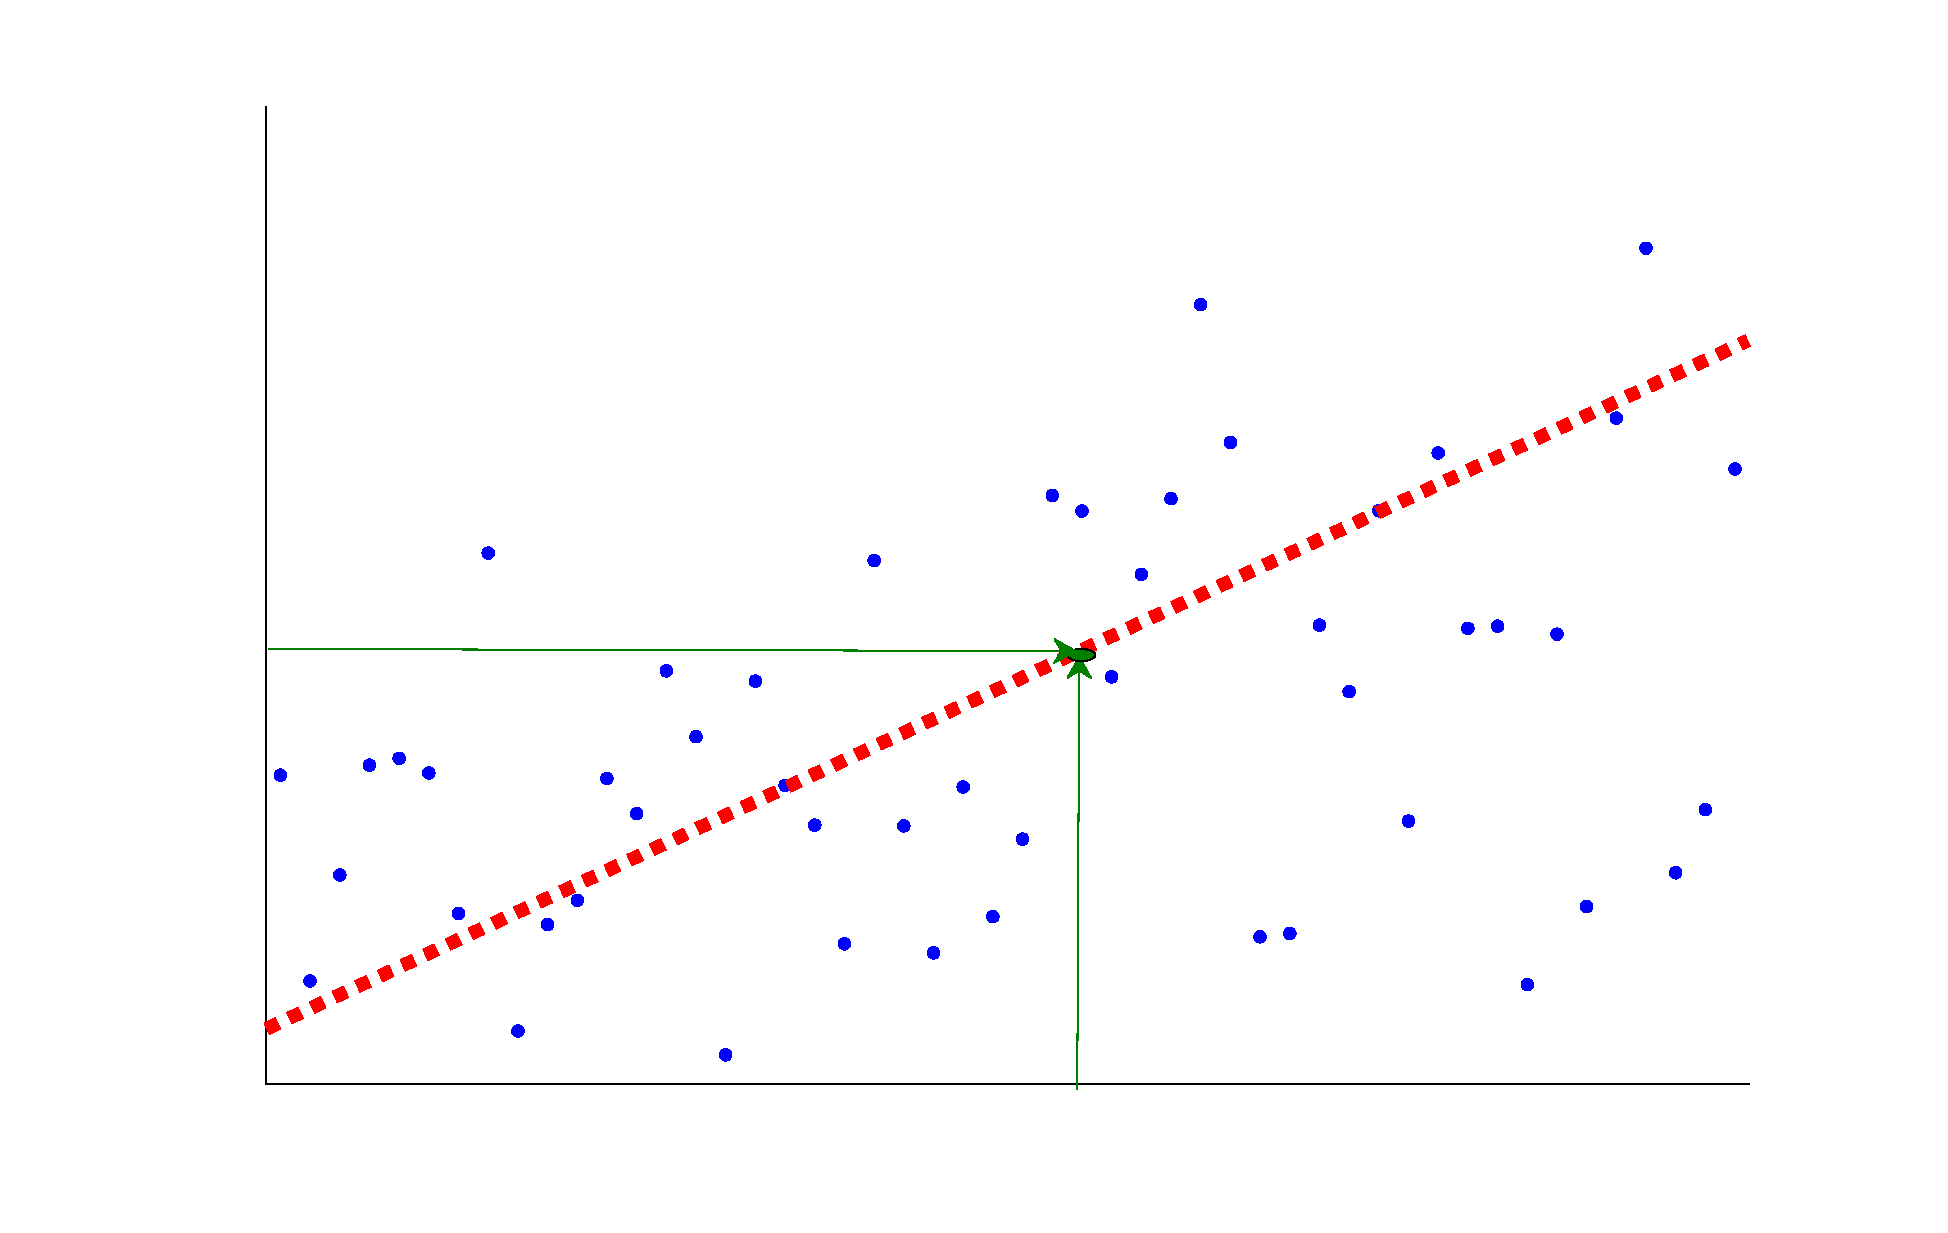
\includegraphics[scale=.35]{pt-est}
  \caption[Scatterplot and OLS Regression]{Scatterplot and OLS regression showing a single point estimate which is at the ($x$, $y$) coordinates marked by arrows.}
  \label{figure:pt-est}
\end{figure}

\subsubsection{Interval Estimation}\index{Interval Estimation}
Interval estimation is the use of sample data to calculate an interval of probable values of an unknown population parameter. The most prevalent forms of interval estimation are \emph{confidence intervals}. Because samples are taken from a population with a distribution, such as a normal distribution (Figure~\ref{figure:pdf}), it is possible that the sample does not accurately describe the population. If a point estimate is taken from one of the two tails of the distribution, it certainly would not represent the mean of the population.

An interval estimate provides some information about the accuracy of the sample and it represents a range of likely values. For instance, we can obtain a 95\% confidence interval, meaning that we have a 95\% confidence that our population mean $\mu$ is contained in our interval. To create the interval we calculate,
\begin{eqnarray}
P \big(-z< \frac{\bar{Y}-\mu}{1/\sqrt{n}}<z \big)&=&.95 ; z= 1.96 \label{eq:conf-int} \\
P \big(-1.96< \frac{\bar{Y}-\mu}{1/\sqrt{n}}<1.96 \big)&=&.95 \notag
\end{eqnarray}
which gives us an interval estimate of $[\bar{y}-1.96/\sqrt{n},\bar{y}+1.96/\sqrt{n}]$, or $\bar{y} \pm 1.96/\sqrt{n}$.

\subsubsection{Hypothesis Testing}\index{Hypothesis Test}\label{hyp-test}
A hypothesis test is a method of making statistical decisions about experimental data that answers the question of how well the findings fit the probability that chance factors alone might be responsible. This is done by asking a hypothetical question and performing a test that compares a sample to its population.

To set up a hypothesis test, we begin with a \emph{null hypothesis}. For example, we want to test a cereal-filling machine at a factory \cite[pp. 332--358]{levine-2004sme}. Our test is to determine if the machine is pouring out the expected weight of 368 grams into each box of cereal.

We have a sample of 25 cereal boxes, and we want to test if the machine is filling properly based on the average weight from our sample. To do so, we must state a null hypothesis,
\[
H_0 : \mu=368,\index{Null Hypothesis}\index{H0@$H_0$|see{Null Hypothesis}}
\]
and an alternative hypothesis as,
\[
H_1 : \mu \ne 368. \index{Alternative Hypothesis}\index{H1@$H_1$|see{Alternative Hypothesis}}
\]

The cereal in the 25 boxes is weighed, and its average (\emph{mean} weight) is found to be 372.5 grams. We know that, on average, the machine has poured too much cereal, some boxes may have too much, others too little. The real question is, ``Is 372.5 grams per box \emph{close enough} to consider the cereal machine to be working?''

Before we can say what is close enough, we need to know how much variance to expect from the cereal-filling machine, and we need to establish a threshold of how much difference is acceptable. Because we are using only a sample, it is possible to make a testing error. We are given the population standard deviation $\sigma=15$.

\paragraph{Hypothesis Errors.}There are two kinds of hypothesis errors we can make,
\begin{description}
\item[Type I Error] This occurs when rejecting a null hypothesis that should not have been rejected. The probability of a Type I error is defined as the \emph{level of significance}\index{Level of Significance} which uses the symbol $\alpha$.\index{alpha@$\alpha$ (alpha)|see{Level of Significance}}
\item[Type II Error] This occurs when not rejecting the null hypothesis when we should have. The probability of a Type II error is denoted by the symbol $\beta$.\index{beta@$\beta$ (beta)!in hypothesis}
\end{description}

\begin{table}[htbp]
   \centering
   \begin{tabular}{@{} lcc @{}}
      \toprule %\hline
      \multicolumn{3}{r}{Actual State of Population} \\
      \hline
       Decision    & $H_0$ is True & $H_0$ is False\\
      \hline
      Reject $H_0$  & Type I Error & Correct Decision \\
      & Probability: $\alpha$ & Probability: $1- \beta$  \\
      \\
      Do not Reject $H_0$   & Correct Decision  & Type II Error \\
      & Probability: $1-\alpha$ & Probability: $\beta$  \\
      \bottomrule %\hline
   \end{tabular}
   \caption{Hypothesis Testing Errors}
   \label{tab:hyp-test-err}
\end{table}

\marginpar{\begin{small}\begin{flushleft}\textcolor{blue}{Two-sided hypothesis test divides the $\alpha$ equally on both tails.}\end{flushleft}\end{small}}
A hypothesis test can be one-sided or two-sided, depending upon the alternative hypothesis. A two-sided hypothesis is nondirectional, such as $H_1: \theta \ne \theta_0$, which we see in Figure~\ref{figure:rej-region2}. A one-sided hypothesis is only concerned with one direction or the other. The alternative hypothesis $H_1: \theta < \theta_0$ is a \emph{left-directional test}, as seen in Figure~\ref{figure:rej-region}, and $H_1: \theta > \theta_0$ is a \emph{right-directional test}.

Our cereal machine should not pour too much or too little cereal. We have established a two-sided hypothesis test. We will establish our level of significance of .05 or 5\%.

\begin{figure}[t]
  \centering
  \includegraphics[scale=.7]{rej-region2}
  \caption{Two-Sided Region of Rejection}
  \label{figure:rej-region2}
\end{figure}
\begin{figure}[t]
  \centering
  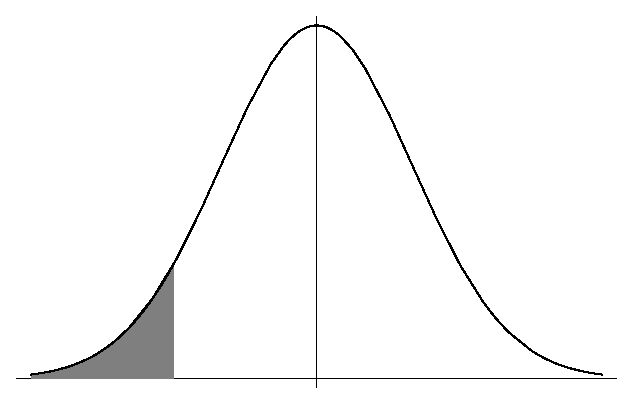
\includegraphics[scale=.7]{rej-region}
  \caption{One-Sided Region of Rejection}
  \label{figure:rej-region}
\end{figure}

Next, we need a \emph{confidence coefficient}, which is denoted by $1-\alpha$. In our cereal test, the confidence coefficient is .95. Our \emph{region of non-rejection} therefore is .95, which implies that our \emph{region of rejection} is .025 on either side of the distribution in Figure~\ref{figure:rej-region2} for a total of .05. We must convert our rejection threshold value into a \emph{critical value} by locating where on the normal distribution the region ending at .025 is located. We can obtain the critical value in MATLAB using,
\ecaption{Obtaining Critical Value}\texttt{cv=norminv((1-0.025),0,1)}, which gives  us 1.96. Since this is a two-tailed test, our critical value is $\pm 1.96$.

Now that we know where the sample mean should lie within the distribution, we need to calculate the \emph{z-test statistic} which determines the sample mean's position relative to the population. The $z$-test statistic is obtained by,
\begin{equation}
\boxed{\quad z = \frac{\bar{X} - \mu}{\frac{\sigma}{\sqrt{n}}}. \quad}
\label{eq:z-test}
\end{equation}
We have the numbers we need to proceed, $\bar{X}=372.5, \mu=368, \sigma=15, n=25$.

We can use \eqref{eq:z-test} to generate a $z$-test statistic,\index{Z@$Z$-Test Statistic}
\[
z = \frac{372.5 - 368}{15/\sqrt{25}} = 1.5.
\]

Since our $z$-test statistic is within the region of non-rejection ($-1.96 < z < 1.96$), we state that there is insufficient evidence to claim that our sample mean is different from the population mean. The difference in the weight of the cereal is ``close enough.''

\subsection{Linear Algebra}\index{Matrix Math|see{Linear Algebra}}\index{Linear Algebra}\index{MATLAB}\index{R language}
To perform matrix operations, We will be using MATLAB, and R, which allow us to perform matrix multiplication and other related operations, but it is important to remember is how to multiply two matrices.
\margincomment{The size of a matrix is described by number of rows $\times$ columns}
For example, matrix $\mathbf{A} \times \mathbf{B}$ where,
\begin{eqnarray}
	\label{eq:matmult}
\mathbf{A} &=& \notag
	\begin{bmatrix}
	1 & 2 & 3 \\
	4 & 5 & 6 \\
	\end{bmatrix} \\
\mathbf{B}&=&  \notag
	\begin{bmatrix}
	10 & 20 \\
	30 & 40 \\
	50 & 60 \\
	\end{bmatrix} \\
\\ \notag
\mathbf{A} \mathbf{B}&=&
	\begin{bmatrix}
	220 & 280 \\
	490 & 640 \\
	\end{bmatrix},
\end{eqnarray}

or, more generally,
\begin{eqnarray}
	\label{eq:matmultnum}
\mathbf{A} &=& \notag
	\begin{bmatrix}
	a_{11} & a_{12} & a_{13} \\
	a_{21} & a_{22} & a_{23} \\
	\end{bmatrix} \\
\mathbf{B}&=&  \notag
	\begin{bmatrix}
	b_{11} & b_{12} \\
	b_{21} & b_{22} \\
	b_{31} & b_{32} \\
	\end{bmatrix} \\
\\ \notag
\mathbf{A} \mathbf{B}&=&
	\begin{bmatrix}
	a_{11} b_{11} + a_{12} b_{21} + a_{13} b_{31} & a_{11} b_{12} + a_{12} b_{22} + a_{13} b_{32} \\
	a_{21} b_{11} + a_{22} b_{21} + a_{23} b_{31} & a_{21} b_{12} + a_{22} b_{22} + a_{23} b_{32} \\
	\end{bmatrix}.
\end{eqnarray}

Only matrices of specific sizes may be multiplied.

The multiplication in \eqref{eq:matmult} and \eqref{eq:matmultnum} is allowed because $\mathbf{A}$ is a $2 \times 3$ matrix, $\mathbf{B}$ is a $3 \times 2$ matrix, and the number of columns in $\mathbf{A}$ must equal the number of rows in $\mathbf{B}$. The expression,
\[
\mathbf{A_{[m \times n]}} \times \mathbf{B_{[p \times q]}}
\]
requires that $n=p$. The resulting matrix will be of size $[m \times q]$.

It is important to note that the order the two matrices is multiplied is very important. The result will most likely be very different, if it can be computed at all.
\margincomment[red]{The law of commutativity does \emph{not} apply to matrices.}
\[
\mathbf{AB} \neq \mathbf{BA}
\]

Often, some calculations require a matrix to be \emph{transposed}. This is simply a rotation of columns to rows, as in the example,
\begin{eqnarray}
\mathbf{A} &=& \notag
	\begin{bmatrix}
	a_{11} & a_{12} & a_{13} \\
	a_{21} & a_{22} & a_{23} \\
	\end{bmatrix} \\
\mathbf{A^{T}} &=& \notag
	\begin{bmatrix}
	a_{11} & a_{21} \\
	a_{12} & a_{22} \\
	a_{13} & a_{23} \\
	\end{bmatrix}
\end{eqnarray}

Let us examine how MATLAB evaluates \eqref{eq:matmult}. A data structure, such as an array or matrix, is enclosed within brackets. The data elements may be comma-separated or separated by a space. A semicolon delimits a new row.
\ecaption{Matrix Multiplication}
\begin{verbatim}
    A=[1 2 3; 4 5 6];
    B=[10 20; 30 40; 50 60];
    A*B

    ans =
       220   280
       490   640
\end{verbatim}
Compare \eqref{eq:matmult} to the MATLAB syntax above to see how the expression is coded. The semicolon at the end of a line suppresses printing of an expression to the Command Window, but the values are displayed in the Workspace.
